%
% FH Technikum Wien
% !TEX encoding = UTF-8 Unicode
%
% Erstellung von Master- und Bachelorarbeiten an der FH Technikum Wien mit Hilfe von LaTeX und der Klasse TWBOOK
%
% Um ein eigenes Dokument zu erstellen, müssen Sie folgendes ergänzen:
% 1) Mit \documentclass[..] einstellen
%    * Master- oder Bachelorarbeit
%    * Studiengang
%    * Sprache (english, german, ngerman)
%    * Zitationsstandard (Harvard, IEEE) (Standard: IEEE)
%    * Biber oder BibTeX als Literaturbackend (Biber, BibTeX) (Standard: Biber)
% 2) Deckblatt, Kurzfassung, etc. ausfüllen
% 3) und die Arbeit schreiben (die verwendeten Literaturquellen in Literatur.bib eintragen)
%
% Getestet mit TeXstudio mit Zeichenkodierung utf-8 (=ansinew/latin1) und TexLive unter Ubuntu
% Zu beachten ist, dass die Kodierung der Datei mit der Kodierung des paketes inputenc zusammen passt!
% Die Kodierung der Datei twbook.cls MUSS ANSI betragen!
% Bei der Verwendung von UTF8 muss nicht nur die Kodierung des Dokuments auf UTF8 gestellt sein, sondern auch die des BibTex-Files!
%
% Bugreports und Feedback bitte per E-Mail an latex@technikum-wien.at
%
% Version V2.24 von 2024-12-19 otrebski
%
\documentclass[MAI,Projekt,english,IEEE]{twbook}%\documentclass[Bachelor,BMR,ngerman]{twbook}
\usepackage[utf8]{inputenc}
\usepackage[T1]{fontenc}

\addbibresource{Literatur.bib}
%% Definieren Sie hier bei Bedarf weitere Literaturdatenbanken

% Die nachfolgenden Pakete stellen sonst nicht benötigte Features zur Verfügung
\usepackage{blindtext}
\usepackage{parskip}  % automatically removes indent and adds vertical space
\usepackage{float}         % für [H], optional
%
% Einträge für Deckblatt, Kurzfassung, etc.
%
\title{Enhancing financial forecasting by sentiment analysis}
\author{David Höchtl BSc.}
\studentnumber{2410585053}
%\author{Titel Vorname Name, Titel\and{}Titel Vorname Name, Titel}
%\studentnumber{XXXXXXXXXXXXXXX\and{}XXXXXXXXXXXXXXX}
\supervisor{Dr. rer. nat. Sharwin Rezagholi, MSc.}
%\supervisor[Begutachter]{Titel Vorname Name, Titel}
%\supervisor[Begutachterin]{Titel Vorname Name, Titel}
%\secondsupervisor{Titel Vorname Name, Titel}
%\secondsupervisor[Begutachter]{Titel Vorname Name, Titel}
%\secondsupervisor[Begutachterinnen]{Titel Vorname Name, Titel}
\place{Wien}
\kurzfassung{\blindtext}
\schlagworte{Schlagwort1, Schlagwort2, Schlagwort3, Schlagwort4}
\outline{\blindtext}
%\acknowledgements{\blindtext}

\begin{document}

\maketitle
\chapter{Abstract}
Financial markets are highly complex systems that are influenced by human behaviours and economic events. For decades, data scientists and economists have attempted to predict and explain financial time series, but it still remains a big challenge. Traditionally, autoregressive models or technical indicators were used to achieve this goal. While this approach created a mathematical and statistical foundation, it falls short when confronted with unstructured data like news headlines or investor sentiment.

With the rapid advances in artificial intelligence (AI), especially in natural language processing (NLP), new ways for understanding those unstructured texts have been found. For example, transformer models can extract semantic information from text. This information could be used to engineer new features that help explain variance in the movement of stock market indices like the S\&P500 or the MSCI World. 

The goal of this master thesis, therefore, is to investigate if a stochastic forecasting approach can be improved by adding sentiment-based features extracted from news headlines and/or social media posts. This feature can be understood as an indicator (usually ranged between -1 and 1), that tries to reflect the emotions of investors towards the current economy. In the scope of a single headline it captures how optimistic (bullish) or pessimistic (bearish) the context appears.

As a proof of concept (PoC), the work will analyse an ARMA model with and without sentiment integration. Later, more complex AI models – ranging from XGBoost to recurrent neural networks (RNNs), long short-term memory networks (LSTMs), and state-of-the-art transformer models like GPT – 5 may be evaluated and benchmarked. To analyse performance, metrics such as Mean Percentage Error (MPE), Accuracy, and F1-Score will be used.

This investigation contributes to an ongoing debate about the efficient market hypothesis, which states that new information is integrated into prices almost instantly, rendering the information useless for predicting future movements.

\chapter{Motivation}
Despite decades-long research in terms of stock predictions, the forecasting of short-term movements remains a challenge. Traditional methods depend solely on previous price movements and technical indicators. However, the influential factors that move the market go far beyond this information. News, Social Media, politics, macro-economic events are examples that could contribute to changes in the stock market as well.

Current studies \cite{ANBAEEFARIMANI2022108742} increasingly work with the analysis of media texts to achieve additional prediction-accuracy, though, the quantitative value of these features is debated. Additionally, the interaction between technical indicators and sentiment features — and their impact on model performance across different AI architectures — remains an open question.

\chapter{Literature Review}
The idea to combine market sentiment with stochastic and technical indicators is not new. Many studies have already done research on it \cite{ANBAEEFARIMANI2022108742} \cite{10380556} \cite{9175549}. The combination of sentiment and well known indicators like ADI (divergences between the price and the volume), volume, EMA (weighted moving average) are used in \cite{ANBAEEFARIMANI2022108742} to predict the price changes in Forex (Foreign exchange markets), with good performance. Similarly \cite{9175549} tried using daily aggregated sentiment and stock-data(isn´t further explained) to predict price changes of certain companies like Apple, Amazon or Microsoft. Both works have proven a correlation between stock price and sentiment, which lead to increased model performance. Also noteable is that \cite{ANBAEEFARIMANI2022108742} stated that specifically combining both technical indicators and sentiment lead to the most performant model, hinting possible feature synergies or complimentations.

However, newspaper headlines are not the only reliable source, social media posts (e.g. twitter or social hubs) can also be utilized to create sentiment features. For example \cite{CHOI2024121589} used properties like views, likes, dislikes, and keywords to predict price momentum (up, down). Other studies like \cite{khan2022stock} even go a step further by combining both news paper headlines with social media content to create more robust accuracy.

In comparison to others this study will focus not on single companies or foreign exchange markets but broad stock indices. On might argue that sentiment analysis is more effective for indices because it reflects more macroeconomic factors. However, the opposite could also be true. Headlines related to a specific company (not included by the index) may introduce noise into the aggregated sentiment score, potentially reducing predictive power. Comparing the outcome of this study with the related ones may give new insights on this topic.

\chapter{Proposed Methods}
The fundamental data of this work will be a big corpus of news paper headlines, that combine multiple American media sources (CNBC, Reuters, The Guradians, ...). A pipeline that combines many of those datasets will be implemented. Primary goal ist to unify many different datasets, remove duplicates and create a time series with news information.
On the other hand using investpy or other public APIs (Alpha Vantage) stock and volume data will be collected for the target index. The frequency will be adjusted for the granuality of the sentiment data (for example an intra day sentiment score is only possible if enough data can be collected).

\section{Example Features Matrix}
Sentiment scores will be genreated with different algorithms and models to compare the effect on performance and stability. Starting from "primitive" tools like lexicon based analysis to state of the art fine tuned transformer models like FinBERT or LLMs like GPT-5. Technical indicators will be calculated from the past price and volume data as part of the feature matrix pipeline. A possible matrix could look like this:

\begin{table}[H]
\centering
\caption{Possible Feature Matrix}
\begin{tabularx}{\textwidth}{l X}
\hline
\textbf{Feature} & \textbf{Description} \\ 
\hline
\textbf{Close Price / Price Change} & 
The price of a fincial instrument at the end of each trading day / The price change that measures the relative or absolute change to prior days \\
\hline
\textbf{Volume} & 
Trading volume shows how many shares have been traded in a give time interval \\
\hline
\textbf{Exponential Moving Average (EMA)} & 
Moving Average that assignes greater weight to newer data points \\
\hline
\textbf{Average True Range (ATR)} &
Measues volatility over a specific time period. \\
\hline
\textbf{Williams \%R} & 
A momentum indicator that indicates whether a stock is overbought (around 0) or oversold (around -100). \\
\hline
\textbf{Accumulation/Distribution Indicator (ADI)} & 
An indicator that combines price and volume data to determine the capital flow into a stock. \\
\hline
\textbf{Sentiment Score} & 
daily aggregated score, that tries to predict market sentiment \\
\hline
\end{tabularx}
\end{table}

(Disclaimer: The provided feature matrix is only an idea. Both technical indicators and sentiment features can/will be changed)

\section{Example Metrics and Statistical Tests}
For regression forecasting tasks (price changes), the following metrics can be used: \textbf{Mean Percentage Error (MPE)}, \textbf{Mean Absolute Error (MAE)}

When predicting directional movements (up, down), the following classification metrics can be applied: \textbf{Accuracy}, \textbf{Precision}, \textbf{Recall}, \textbf{F1-Score}

To validate whether sentiment features have a statistically significant impact on model performance, the following tests could be used: \textbf{p-Value Test}, \textbf{Granger Causality Test}

\section{Goal and Milestones}
The goal of this study is to quantify the benefit of market-sentiment to predict changes in stock prices. Different AI-algorithms will be compared and analysed to determine which would benefit the most from this new feature. Following milestone list will outline the work:

\begin{table}[H]
\centering
\caption{Goals Milestone Plan}
\label{tab:milestones}
\begin{tabular}{|c|p{9,5cm}|p{1,5cm}|c|}
\hline
\textbf{Week / Month} & \textbf{Task} & \textbf{Status} \\
\hline
Week 1--2 (Sept) & Start with Literature Review and scouting for the first prototyp datasets of news headlines & Done \\
\hline
Week 3--4 (Sept) & Create a simple sentiment pipeline that classifies news headlines. Analyse different finance APIs that can provide daily prices for finacial trackers & Done \\
\hline
Week 5--6 (Oct) & Use the gathered an prepared data to train ARMA Models and compare the effect of adding the sentiment feature. (first prototype) & Done \\
\hline
Week 7--10 (Oct/Nov) & Create a pipeline that can combine different dataset, gather more data and try around with different sentiment lags (analyse the decay of explainability over time) / compare sentiment models (lexicon -> transformer) & Pending \\
\hline
Week 11--12 (Nov) & Create pipeline that calculates technical indicators and combine them with the sentiment scores to create a complete feature Matrix & Pending \\
\hline
Week 13--16 (Dec) & Model training and evaluation (ARMA, XGBoost, RNN, LSTM, GPT) Evaluation metrics (MPE, Accuracy, F1-Score) & Pending \\
\hline
Week 17--18 (Jan) & feature contirbution analysis, performance comparision and preparation of presentation & Pending \\
\hline
Week 19--20 (Jan) & buffer & - \\
\hline
\end{tabular}
\end{table}

\chapter{First prototype}
In the course of a minimal experiment, ARIMA-Models produced hints that sentiment has a statistical value for predicitng prices. For this purpose, an autoregressive (AR) model with a moving average (MA) component was used. ARIMA models are primary used in statistic and economic szenarios. It is important to note that, in this case the previous proposed matrix was not used. Instead only price and sentiment of prior N days where utilized for predicting future values.

A ARIMA(p,d,q) model has 3 different parameter \cite{WikipediaARIMA}:
\begin{itemize}
    \item p => N past datapoints (t-1, t-2, ... t-n)
    \item d => degree of differencing, makes changes stationary (e.g., from price movement to price change)
    \item q => N past regression errors
\end{itemize}

\section{Setup}

\begin{table}[H]
\centering
\caption{Setup of the experiment}
\begin{tabularx}{\textwidth}{l X}
\hline
\textbf{Model} & 
Arima(1,0,1) vs ARIMA (1,0,1) + daily aggregated sentiment \\
\hline
\textbf{Dataset} & 

- Kaggle dataset (CNBC, Retuers, The Guardians - headlines) covering ~01.01.2018 - ~16.07.2020 \cite{LucasPhamFinDataset}

- daily prices of the S\&P500 (US) in the same time range via investpy API

(648 data points) \\

\hline
\textbf{Sentiment Model} & 
Vader Lexikon \\
\hline
\textbf{Benchmark} &
AIC, BIC \\
\hline
\end{tabularx}
\end{table}

\section{Results}
\begin{figure}[H]
    \centering
    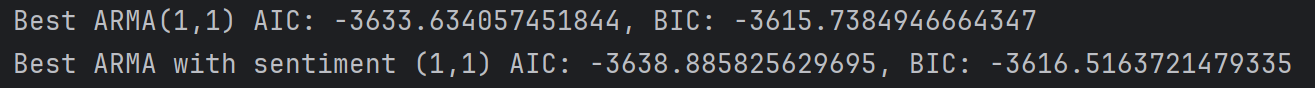
\includegraphics[width=0.9\textwidth]{PICs/ARMA101_Result.png}
    \caption{AIC and BIC Benchmark}
    \label{fig:myimage}
\end{figure}

Both AIC and BIC shrink with the addition of sentiment score. Even though the difference is small, this experiment provide valuable insights that sentiment can contribute positive to model performance.

\begin{figure}[H]
    \centering
    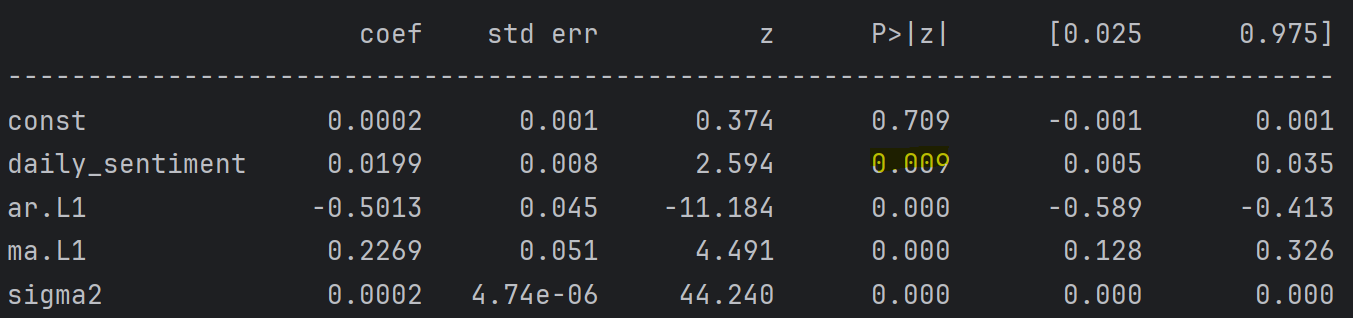
\includegraphics[width=0.9\textwidth]{PICs/ARIMA101_sentiment_p_value.png}
    \caption{Feature list ARMA(1,0,1) with sentiment}
    \label{fig:myimage2}
\end{figure}

The low p-value proves that the feature daily\_sentiment is statistical significant

While this results are very promising following two challenges were indentified. First, while the ARMA sentiment model generally outperformed the ARMA mdoel, this was not the case for every configuration. Second for the year 2018, no significant relationship between sentiment and price movement could be proven (p-value \= 0.457). Therefore, although this experiment is an important indicator that sentiment explains some variance, more data and further investigations are needed to find clear answers.

\chapter{Example Plots}
\begin{figure}[H]
    \centering
    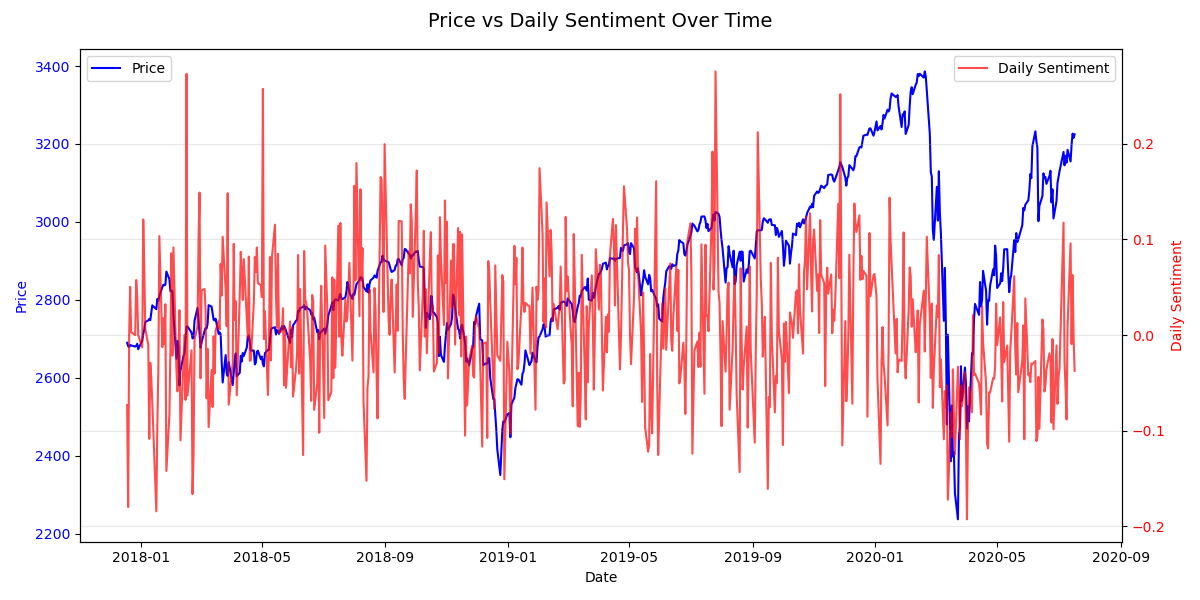
\includegraphics[width=1\textwidth]{PICs/Example_plot_sentiment_price.png}
    \caption{Sentiment vs Price}
    \label{fig:myimage3}
\end{figure}

\begin{figure}[H]
    \centering
    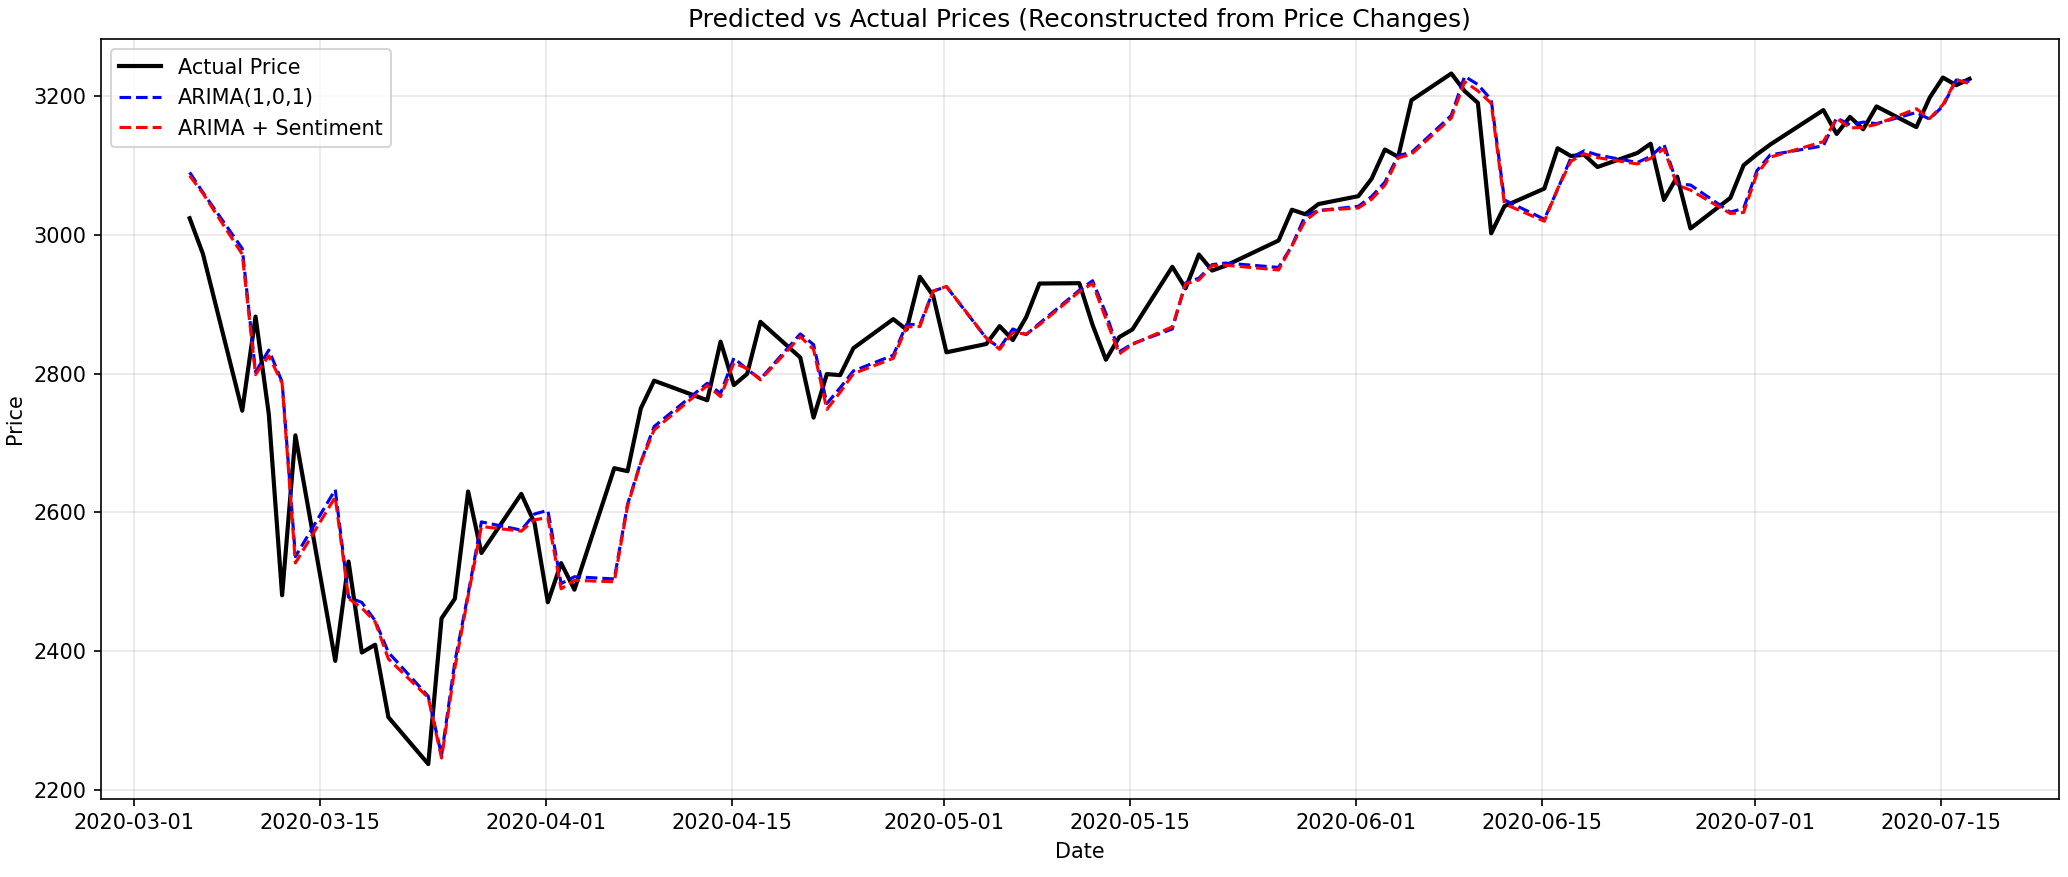
\includegraphics[width=1\textwidth]{PICs/Example_plot_prediction_vs_actual.png}
    \caption{Predicted vs Actual Prices}
    \label{fig:myimage4}
\end{figure}
%
% Hier beginnen die Verzeichnisse.
%
\clearpage
\printbibliography
\clearpage

% Das Abbildungsverzeichnis
\listoffigures
\clearpage

% Das Tabellenverzeichnis
\listoftables
\clearpage

\end{document}
